We investigated three versions of the AWP design described in the last section of the previous chapter. The first type we present is based on 3D printed \ce{Al2O3}, the second type is produced using ordinary 3D printed polymers and the third type consists of SLE fused silica glass waveplates as described in the previous chapter. The results are obtained through the minimization of the two objective functions defined in the previous chapter.

% This AWP type differs from the other two in the sense that the phase shift is not caused by form birefringence, but instead by intrinsic birefringence which stems from the crystallographic orientation of the material. The second type is similar to the fused silica glass AWP in the sense that it is also based on form birefringence but the structure is 3D printed by typical of the birefringence is not from the structure but instead on the crystallographic orientation of the material. 

\section{Ceramic AWP}
In a publication by Ornik et al. it was shown that \ce{Al2O3} as a 3D printed ceramic exhibited birefringent properties. A birefringence of approximately $0.05$ was reported. This value is fairly low compared to the birefringence of sapphire which is the crystalline form of \ce{Al2O3} with a birefringence of approximately $0.32$. 

\begin{figure}[h]
    \centering
    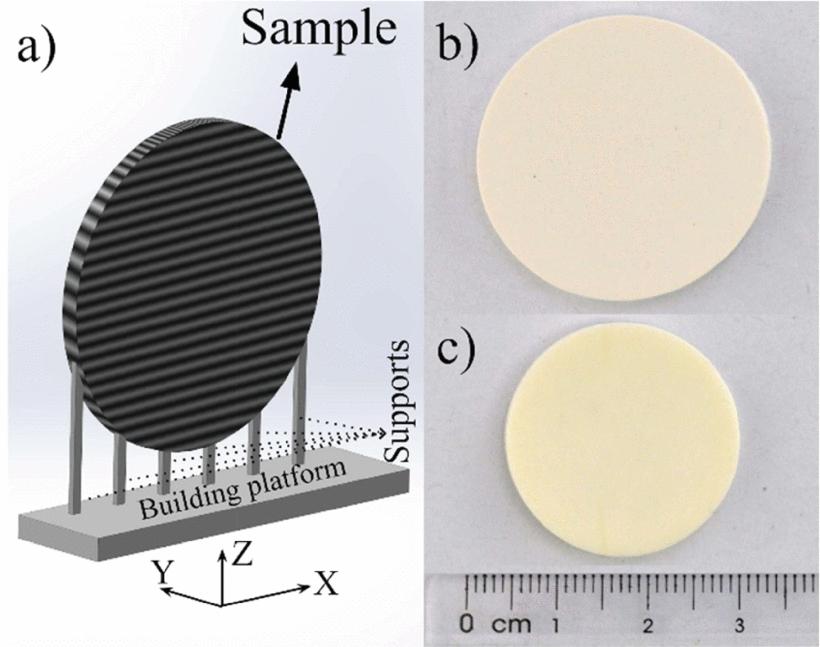
\includegraphics[scale=0.4]{images/5_chapter05/ornik1abc-3047514-large.png}
    \caption{Schematic image of the a) printed sample as well as photographs of b) green and c) sintered Alumina. Source: \cite{Ornik2021}}
    \label{fig:ornik1abc}
\end{figure}

It was further shown that the direction of the slow axis was parallel to the printing direction. A sketch of how the samples are printed is shown to the left in figure \ref{fig:ornik1abc}, where the arrow indicates the printing direction. The top right side shows an actual image of the green sample and the bottom right shows an image of the sample after sintering. For the sintering step the sample is slowly heated to \SI{1700}{\celsius} which causes it to shrink, in this case by around \SI{21}{\volpercent}. In total two different samples were characterized and the result of this characterization is shown in figure \ref{fig:ri_abs} \cite{Ornik2021}. The left plot shows the measured refractive index and the birefringence along the slow and fast direction for the two samples as a function of the frequency, while the right plot shows the measured absorption coefficient for the two samples and directions as a function of the frequency. We see that within the error range the birefringence of the two samples is equal. Therefore, either sample parameters works for setting up the loss function, we use the measurement result from sample 1. 

\begin{figure}[h]
    \centering
    \includestandalone[scale=0.73]{5_chapter05/plots/ceramic/ri_bf}
    \caption{}
    \label{fig:ri_abs}
\end{figure}

Stacking a number of these ceramic discs or plates like the one shown in figure \ref{fig:ornik1abc} we can in theory construct an AWP similar to the TAQ by Masson. This ceramic AWP can then serve as a comparison to the TAQ and therefore also partly as a verification of the loss function at least for the $\lambda/4$ AWP type. In this case the loss functions $L_{\lambda/4}$ and $L_{\lambda/2}$ only depend on the set of angles and thicknesses. In other words the birefringence does not change at each iteration during optimization and is the same for each individual plate. 

\begin{table}[h]
    \centering
    \includestandalone{5_chapter05/ceramic_result_table}
    \caption{}
    \label{tab:ceramic_result_l4}
\end{table}

\subsection{Simulation}
\subsection{CST}
\subsection{Fabrication error}

\section{Polymer}

\section{Fused silica glass}

% Todo ref?


